\documentclass[12pt,a4paper,oneside]{book} 

%%%%%%%%%%%%%%%%%%%%%%%%%%%%%%%%%%%%%%%%%%%%%%%%%%%%%%%%%%%%%%%%%%%%%%%%

\usepackage{ifthen}
\usepackage{graphicx}
\usepackage[dvips]{epsfig}
\usepackage{enumerate}
\usepackage{calc}
\usepackage{multicol} 
\usepackage{titlesec}
%\usepackage{showkeys}

%%%%%%%%%%%%%%%%%%%%%%%%%%%%%%%%%%%%%%%%%%%%%%%%%%%%%%%%%%%%%%%%%%%%%%%%

\usepackage{a4}
\usepackage{amsfonts}
\usepackage{amssymb}
\usepackage{epsfig}

%%%%%%%%%%%%%%%%%%%%%%%%%%%%%%%%%%%%%%%%%%%%%%%%%%%%%%%%%%%%%%%%%%%%%%%%

\usepackage{t1enc,times}
\usepackage{latexsym,amssymb}
\usepackage{amsmath}
\usepackage{amstext}
%\usepackage[T1]{fontenc}
%\usepackage{cmbright}
\usepackage{pifont}
\usepackage{marvosym}
%\usepackage{pslatex}
% \usepackage{stmaryrd} %=== > dont have it installed on system, doesnt look like it's a compulsory package anyway
%\usepackage{txfonts}  

%%%%%%%%%%%%%%%%%%%%%%%%%%%%%%%%%%%%%%%%%%%%%%%%%%%%%%%%%%%%%%%%%%%%%%%%%%%%%%%
\usepackage[titletoc]{appendix}
%%%%%%%%%%%%%%%%%%%%%%%%%%%%%%%%%%%%%%%%%%%%%%%%%%%%%%%%%%%%%%%%%%%%%%%%%%%%%%%

\usepackage{fancybox} 
\usepackage{fancyhdr}
\usepackage{fullpage}

%%%%%%%%%%%%%%%%%%%%%%%%%%%%%%%%%%%%%%%%%%%%%%%%%%%%%%%%%%%%%%%%%%%%%%%%%%%%%%%

%\usepackage{url}    
%\ExecuteOptions{dvips}
%\usepackage[pdftex,colorlinks=true]{hyperref}
%\hypersetup{backref,pdfpagemode=UseThumbs,pdfstartview=Fit,
%pdfpagelayout=SinglePage,pdfstartpage=1,colorlinks=true,menucolor=msc,
%anchorcolor=msc,pagecolor=msc,urlcolor=rfr,breaklinks=true,hyperfootnotes=true}

%%%%%%%%%%%%%%%%%%%%%%%%%%%%%%%%%%%%%%%%%%%%%%%%%%%%%%%%%%%%%%%%%%%%%%%%%%%%%%%

\pagestyle{fancy}
\fancyhf{} 
%\renewcommand{\headrulewidth}{1pt}
%\renewcommand{\footrulewidth}{1pt}
\renewcommand{\headwidth}{\textwidth}
\fancyhead[LE]{\leftmark}
\fancyhead[RO]{\small \rightmark}
\fancyfoot[C]{\thepage}

%%%%%%%%%%%%%%%%%%%%%%%%%%%%%%%%%%%%%%%%%%%%%%%%%%%%%%%%%%%%%%%%%%%%%%%%%%%%%%%

\tolerance 4000
\textwidth 17.00cm
\topmargin -0.30cm
\oddsidemargin -0.25cm
\evensidemargin -0.25cm
\textheight 23.00cm
%\headsep 12pt
\headheight 15pt
\footskip 60pt
%\parindent 12pt

%%%%%%%%%%%%%%%%%%%%%%%%%%%%%%%%%%%%%%%%%%%%%%%%%%%%%%%%%%%%%%%%%%%%%%%%%%%%%%%

\renewcommand{\rmdefault}{ptm}  % times
\renewcommand{\rmdefault}{phv}  % helvetica
\renewcommand{\rmdefault}{pbk}  % bookman
\renewcommand{\rmdefault}{ppl}  % palatino
\renewcommand{\sfdefault}{phv}  % helvetica as sans serif
\renewcommand{\ttdefault}{pcr}  % courier as fixed width
\renewcommand{\tabcolsep}{8pt}
\renewcommand{\arraystretch}{1.25}

%%%%%%%%%%%%%%%%%%%%%%%%%%%%%%%%%%%%%%%%%%%%%%%%%%%%%%%%%%%%%%%%%%%%%%%%%%%%%%%

\def\nn{\nonumber}
\def\f{{\frac}}
\def\pa{{\partial}}
\def\d{{\rm d}}
\def\l{\left}
\def\r{\right}
\def\Mpl{M_{_{\rm Pl}}}

%%%%%%%%%%%%%%%%%%%%%%%%%%%%%%%%%%%%%%%%%%%%%%%%%%%%%%%%%%%%%%%%%%%%%%%%%%%%%%%

\def\done{\marginpar {\scriptsize DONE}}
\def\check{\marginpar {\scriptsize CHECK}}

%%%%%%%%%%%%%%%%%%%%%%%%%%%%%%%%%%%%%%%%%%%%%%%%%%%%%%%%%%%%%%%%%%%%%%%%%%%%%%%

\begin{document}

%%%%%%%%%%%%%%%%%%%%%%%%%%%%%%%%%%%%%%%%%%%%%%%%%%%%%%%%%%%%%%%%%%%%%%%%%%%%%%%

\baselineskip 20pt

%%%%%%%%%%%%%%%%%%%%%%%%%%%%%%%%%%%%%%%%%%%%%%%%%%%%%%%%%%%%%%%%%%%%%%%%%%%%%%%

\pagenumbering{roman}

%%%%%%%%%%%%%%%%%%%%%%%%%%%%%%%%%%%%%%%%%%%%%%%%%%%%%%%%%%%%%%%%%%%%%%%%%%%%%%%

\thispagestyle{empty}
\topskip 15pt
\hrule\hrule\hrule\hrule\hrule
\vskip 20pt
\centerline{\Huge \bf Generation of Gravitational waves} 
\vskip 15pt
\centerline{\Huge \bf during Inflation.} 
\vskip 20pt
\hrule\hrule\hrule\hrule\hrule
\vskip 30pt
\centerline{\Large A mini-project report}
\vskip 8pt
\centerline{\Large submitted in partial fulfilment 
for the award of the degree of}
\vskip 8pt
\centerline{\Large B.S \& M.S in Physics}
%\vskip 8pt
%\centerline{\Large in}
%\vskip 8pt 
%\centerline{\Large Physics}
\vskip 8pt
\centerline{\Large by}
\vskip 8pt
\centerline{\Large \bf Poruri Sai Rahul}
\vskip 8pt
\centerline{\Large under the guidance of}
\vskip 8pt
\centerline{\Large  Dr.~L.~Sriramkumar}
\vskip 30pt 
\begin{center}

\epsfig{file=iitm.eps, width=3.0cm, height=3.0cm} % needed to convert .ps ext to .eps ext.
\end{center}
\vskip 8pt 
\centerline{\Large \bf Department of Physics}
\vskip 8pt 
\centerline{\Large \bf Indian Institute of Technology Madras}
\vskip 8pt 
\centerline{\Large \bf Chennai~600036, India}
\vskip 8pt
\centerline{\Large \bf June~2015}
%%%%%%%%%%%%%%%%%%%%%%%%%%%%%%%%%%%%%%%%%%%%%%%%%%%%%%%%%%%%%%%%%%%%%%%%%%%%%%%

\newpage\topskip 40pt
\centerline{\Large CERTIFICATE}
\thispagestyle{empty}
\vskip 20pt\noindent 
This is to certify that the project titled {\bf Generation of Gravitational
waves during Inflation} is a bona fide record of work done by 
{\bf Poruri Sai Rahul} towards the partial fulfilment of the 
requirements of the B.S \& M.S degree in Physics at the Indian 
Institute of Technology, Madras, Chennai 600036, India.
\vskip 120pt
\hspace{240pt}(L.~Sriramkumar, Project supervisor)

%%%%%%%%%%%%%%%%%%%%%%%%%%%%%%%%%%%%%%%%%%%%%%%%%%%%%%%%%%%%%%%%%%%%%%%%%%%%%%%

\newpage\topskip 40pt
\thispagestyle{empty}
\centerline{\Large ACKNOWLEDGEMENTS}
\vskip 20pt\noindent 

I cannot express in words my gratitude to {\bf Dr. L.~Sriramkumar} 
for guiding me, regarding my work and my personal life. I would also
like to thank V.~Sreenath and Debika Choudhury for helping me 
with my project and for clarifying my doubts.

A big shout out to my family and my friends, especially Shashi Kunwar
and Preeti Saryan, who have kept me on my toes over the last few years.
 
 %%%%%%%%%%%%%%%%%%%%%%%%%%%%%%%%%%%%%%%%%%%%%%%%%%%%%%%%%%%%%%%%%%%%%%%%%%%%%%%

\newpage\topskip 40pt
\thispagestyle{empty}
\centerline{\Large ABSTRACT}
\vskip 20pt\noindent 

The precision with which inhomogeneities in the Cosmic Microwave Background, CMB for short, are being measured
has increased tremendously over the years, thanks to the efforts of the people behind the Planck and the WMAP 
missions. We are currently in an era of precision cosmology. The theory of inflation predicts the presence of such 
inhomogeneities. In this work, I studied the theory behind the generation and evolution of tensor perturbations, 
otherwise referred to as primordial gravitational waves. I also numerically estimate the power spectrum of such 
perturbations for two different models of inflation.
%%%%%%%%%%%%%%%%%%%%%%%%%%%%%%%%%%%%%%%%%%%%%%%%%%%%%%%%%%%%%%%%%%%%%%%%%%%%%%%

\newpage
\thispagestyle{empty}
\tableofcontents
\newpage

%%%%%%%%%%%%%%%%%%%%%%%%%%%%%%%%%%%%%%%%%%%%%%%%%%%%%%%%%%%%%%%%%%%%%%%%%%%%%%%

\newpage
\thispagestyle{empty}
\listoffigures
\newpage

%%%%%%%%%%%%%%%%%%%%%%%%%%%%%%%%%%%%%%%%%%%%%%%%%%%%%%%%%%%%%%%%%%%%%%%%%%%%%%%

\pagenumbering{arabic}

%%%%%%%%%%%%%%%%%%%%%%%%%%%%%%%%%%%%%%%%%%%%%%%%%%%%%%%%%%%%%%%%%%%%%%%%%%%%%%%

\chapter{Introduction}

\paragraph*{} The big bang theory, proposed in the 1930s, solved the biggest problems at the time i.e the expansion of the universe and 
the presence of a homogeneous thermal CMB radiation. Over time, it was discovered to have some serious drawbacks, the most notable 
of which are the horizon problem and the flatness problem. Introduced in the 1960s, the theory of inflation was successful in solving 
these puzzles and also provided a sound causal mechanism for the generation of inhomogeneities in the CMB, which acted as the seeds 
for large scale structure formation in the universe. For an in-depth discussion of the horizon problem, refer to ~\cite{Sriramkumar L - 2009}.
Inflation commonly refers to a period of rapid expansion of the universe during early stages of the radiation dominated epoch.

\section{Inflaton}

\paragraph*{} A necessary condition for inflation to occur is

\begin{equation}
\ddot{a} > 0
\end{equation}

\noindent and it is straight forward to check that neither matter, for which $a(t) \propto t^{2/3}$, nor radiation, for which , for which $a(t) \propto t^{1/2}$, 
satisfies this condition. We can therefore assume that a generic scalar field $\phi$ and a corresponding potential $V(\phi)$ govern the inflationary 
paradigm. A scalar field that drives inflation is also referred to as an Inflaton.

\paragraph*{} Assuming that a scalar field $\phi$ and a corresponding potential $V(\phi)$ govern the inflationary paradigm, we can write the corresponding action and the stress-energy tensor for the scalar field as

\begin{equation}
S(\phi) = \int d^4x[\frac{1}{2}\partial^{\lambda}\phi \partial_{\lambda}\phi - V(\phi)]
\end{equation}

\begin{equation}
T^{\mu}_{\nu} = \partial^{\mu}\phi \partial_{\nu}\phi -\delta^{\mu}_{\nu}[\frac{1}{2}\partial^{\lambda}\phi \partial_{\lambda}\phi - V(\phi)]
\end{equation}

\noindent We can also derive the equations of motion for the scalar field from the action to be

\begin{equation}
\ddot{\phi} + 3H\dot{\phi} + V_{\phi} = 0
\end{equation}

\noindent where $V_{\phi} = \frac{dV}{d\phi}$

\section{Metric Perturbations}

\paragraph*{} Inhomogeneities in the CMB are one part in $10^5$ and it can be inferred that they should be much smaller at earlier epochs given the expanding nature of our universe. We can therefore study the generation and evolution of such perturbations using linear perturbation theory. While higher-order perturbations have been discovered in recent CMB observations, they are beyond the scope of this work. The linear perturbations in Friedmann-Robertson-Lemaitre-Walker metric, FRLW for short, can be classified as scalar, vector and tensor perturbations, represented as

\begin{equation}
ds^2 = (1+2\Phi)dt^2 - a^2(t)(1-2\Psi)d\bar{x}^2
\end{equation}

\begin{equation}
ds^2 = dt^2 - a^2(t)[\delta_{ij} + (\nabla_iF_j +\nabla_jF_i)]dx^idx^j
\end{equation}

\begin{equation}
ds^2 = dt^2 - a^2(t)(\delta_{ij} + h_{ij})dx^idx^j
\end{equation}

For the scope of this work, I restrict myself to tensor perturbations of the metric, also referred to as gravitational waves, characterized by transverse, traceless matrix $h_{ij}$. The perturbed Einstein equations corresponding to the above metric with tensor perturbations are

\begin{equation}
\delta G^0_0 = \delta G^0_i = 0
\end{equation}

\begin{equation}
\delta G^i_j = -\frac{1}{2}(\ddot{h_{ij}} + 3H\dot{h_{ij}} - \frac{1}{a^2}\nabla ^2h_{ij})
\end{equation}

\noindent In the absence of anisotropic stresses i.e if $\delta T^i_j = 0$, we get that

\begin{equation}
\ddot{h} + 3H\dot{h} - \frac{1}{a^2}\nabla ^2h = 0
\end{equation}

\paragraph*{} Upon quantization, we can write the tensor perturbations $h$ in terms of it's fourier modes $h_k$ as

\begin{equation}
\hat{h}(\eta, \bar{x}) = \int \frac{d^3\bf{k}}{(2\pi)^{3/2}} [\hat{a_k}h_k(\eta)e^{i\bf{k\cdot x}}+ \hat{a_k}^{\dagger}h_k^{*}(\eta)e^{-i\bf{k\cdot x}}] 
\end{equation}

\noindent where the creation and annihilation operators, $\hat{a_k}$ and $a\hat{a_k}^{\dagger}$, follow the standard commutation relations. At the linear order in perturbations that we are working in the power spectrum of the tensor perturbations can be characterized by the two point function of the quantum field $\hat{h}$. The power spectrum of the tensor perturbations $P_T(k)$ and the two point function are related by

\begin{equation}
\int^{\infty}_0 P_T(k) = \int d^3{\bf{k}}\int\frac{d^3(\bf{x}-\bf{x'})}{(2\pi)^3}\langle 0|P(\eta,{\bf{x}})P(\eta, {\bf{x'}})|\rangle \times e^{-i{\bf{k \cdot (x-x')}}}
\end{equation}

\noindent where $|0\rangle$ is the vaccum state defined as $\hat{a_k}|0\rangle = 0 \forall {\bf{k}}$. Using the earlier relation, one can obtain the power spectrum as

\begin{equation}
P_T(k) = 2 (\frac{k^3}{2\pi^2}) |h_k|^2
\end{equation}

\noindent where the factor of 2 is needed to take into account the two states of polarization, $+$ and $\times$, of the gravitational waves.

%%%%%%%%%%%%%%%%%%%%%%%%%%%%%%%%%%%%%%%%%%%%%%%%%%%%%%%%%%%%%%%%%%%%%%%%%%%%%%%

\chapter{Inflationary models}

%%%%%%%%%%%%%%%%%%%%%%%%%%%%%%%%%%%%%%%%%%%%%%%%%%%%%%%%%%%%%%%%%%%%%%%%%%%%%%%

\paragraph*{} Recall that the stress-energy tensor for a scalar field $\phi$ and potential $V(\phi)$ is of the form

\begin{equation}
T^{\mu}_{\nu} = \partial^{\mu}\phi \partial_{\nu}\phi -\delta^{\mu}_{\nu}[\frac{1}{2}\partial^{\lambda}\phi \partial_{\lambda}\phi - V(\phi)]
\end{equation}

\noindent and the individual components can be written as

\begin{equation}
T^{0}_{0} = \partial^{0}\phi \partial_{0}\phi -\delta^{0}_{0}[\frac{1}{2}\partial^{\lambda}\phi \partial_{\lambda}\phi - V(\phi)] = \dot{\phi}^2 -\delta^{0}_{0}[\frac{1}{2}\dot{\phi}^2 - V(\phi)]
 = [\frac{1}{2}\dot{\phi}^2 +V(\phi)] = \rho 
\end{equation}

\begin{equation}
T^{i}_{j} = \partial^{i}\phi \partial_{j}\phi -\delta^{i}_{j}[\frac{1}{2}\partial^{\lambda}\phi \partial_{\lambda}\phi - V(\phi)]
 = -\delta^{i}_{j}[\frac{1}{2}\dot{\phi}^2 - V(\phi)] = -p\delta^i_j
\end{equation}

\paragraph*{} Recall that the einstein's equations corresponding to a smooth FLRW universe result in the following two relations for the scale factor $a(t)$

\begin{equation}
(\frac{\dot{a}}{a})^2 = H^2 = (\frac{8\pi G}{3})\rho
\end{equation}

\begin{equation}
\frac{\ddot{a}}{a} = \dot{H} + H^2= -\frac{4\pi G}{3}(\rho + 3p)
\end{equation}

\noindent where $\rho$ and $p$ correspond to the energy density and pressure of the scalar field driving the inflation.

\paragraph*{} The above equations can be rewritten as

\begin{equation}
 \dot{H} = -H^2 -\frac{4\pi G}{3}(\rho + 3p) = -\frac{4\pi G}{3}3(\rho + p)
= \frac{-1}{2M_P^2}\dot{\phi}^2
\end{equation}

\noindent where I've used the fact that $\frac{1}{M_P^2} = 8\pi G$

\begin{equation}
H^2 = (\frac{1}{3M_P^2})[\frac{\dot{\phi}^2}{2} + V_{\phi}]
\end{equation}

\paragraph*{} By substituting the expressions for $\rho$ and $p$, one can arrive at the following expressions for $\phi(t)$ and $V(t)$.

\begin{equation}
\phi(t)= \sqrt{2}M_P \int dt \sqrt{-\dot{H}}
\end{equation}

\begin{equation}
V(t) = M_P^2(3H^2 + \dot{H})
\end{equation}

\section{Power law inflation}

\paragraph*{} Assuming a power-law form of the scale factor during inflation, of the form

\begin{equation}
a(t) = a_0t^q
\end{equation}

\noindent We can see that the scalar field that drives the inflation has to the of the form

\begin{equation}
\frac{\phi(t)}{M_P} =\sqrt{2q}ln[\sqrt{\frac{V_0}{(3q-1)q}}(\frac{t}{M_P})]
\end{equation}

\begin{equation}
V(\phi) = V_0exp(-\sqrt{\frac{2}{q}}(\frac{\phi}{M_P}))
\end{equation}

%\section{Slow-roll inflation}

%%%%%%%%%%%%%%%%%%%%%%%%%%%%%%%%%%%%%%%%%%%%%%%%%%%%%%%%%%%%%%%%%%%%%%%%%%%%%%%

\chapter{Numerical results}

\paragraph{} In this section, I describe the procedure adopted to numerically evaluate the tensor power spectrum of gravitational waves in a power-law inflationary scenario. Recall that conventionally, e-fold $N$ is defined as $N = log(a/a_0)$, where $N$ gives an estimate of the amount of inflation needed to solve the horizon problem. Also, note that an overdot represents differentiation with respect to coordinate time $t$ and that an overprime represents differentiation with respect to conformal time $\eta$.

\section{Power-law inflation}

\paragraph{} Assuming an inflationary potential $V(\phi)$ of the form

\begin{equation}
V(\phi) = V_0 exp(-(\frac{2}{q})^{1/2}(\phi - \phi_0))
\end{equation}

\noindent where $\phi$ represents the scalar field driving inflation and $q$ is the power-law index.

\paragraph*{} Recall that the equation describing the evolution of the scalar field $\phi$ is

\begin{equation}
\ddot{\phi} + 3H\dot{\phi} + V_{\phi} = 0
\end{equation}

\noindent which can then be written in terms of e-fold time $N$ as

\begin{equation}
\frac{d^2\phi}{dN^2} + (3 - \frac{1}{2}(\frac{d\phi}{dN})^2)\frac{d\phi}{dN} + (6 - (\frac{d\phi}{dN})^2)\frac{1}{2V(\phi)}\frac{dV(\phi)}{dN} = 0
\end{equation}

\noindent Note that I've made used of the following definition for H to arrive at the above expression

\begin{equation}
H^2 = \frac{2V(\phi)}{3-(\frac{d\phi}{dN})^2}
\end{equation}

\paragraph*{} I numerically integrated the above second order differential equation from e-fold time $N = 0$ to $N = 70$ while assuming that $\phi_0 = 1$ and $\frac{d\phi}{dN}_0 = \frac{\sqrt{2q}}{t_0}\frac{1}{H_0}$ using a fourth-order Runge-Kutta method, implemented in Python.

\begin{figure}
\begin{center}
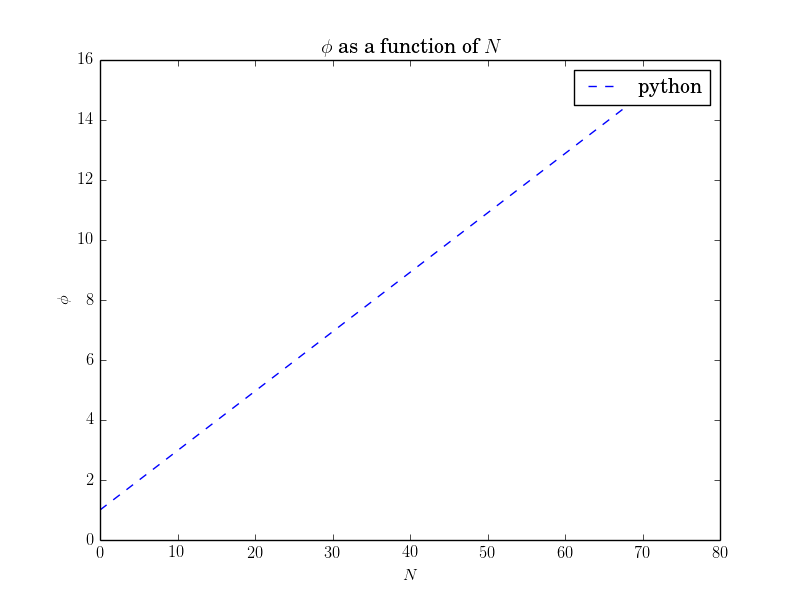
\includegraphics[scale=0.5]{phi_vs_N.png}
\caption[Plot of $\phi(N)$ vs $N$ during power law inflation]{Plot of $\phi(N)$ vs $N$ during power law inflation}
\label{blah}
\end{center}
\end{figure}

\begin{figure}
\begin{center}
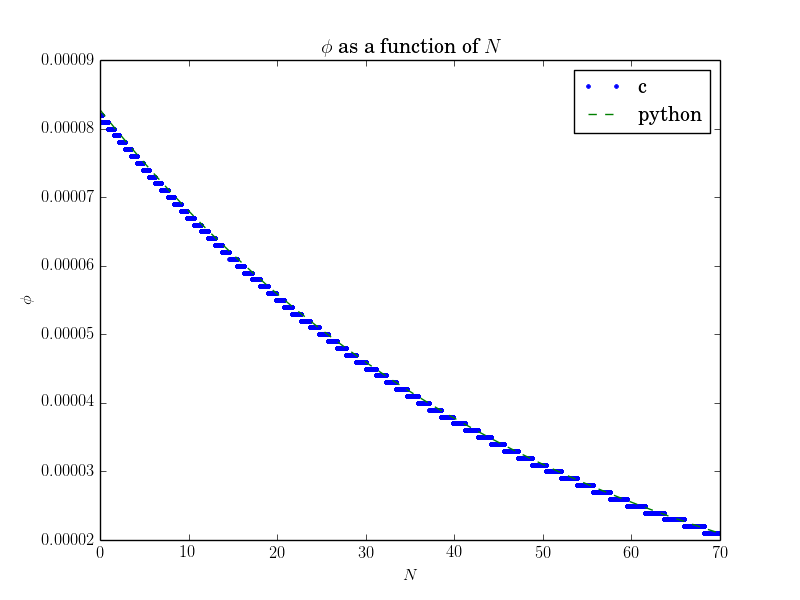
\includegraphics[scale=0.5]{H_vs_N.png}
\caption[Plot of $H(N)$ vs $N$ during power law inflation]{Plot of $H(N)$ vs $N$ during power law inflation}
\label{blah}
\end{center}
\end{figure}

\begin{figure}
\begin{center}
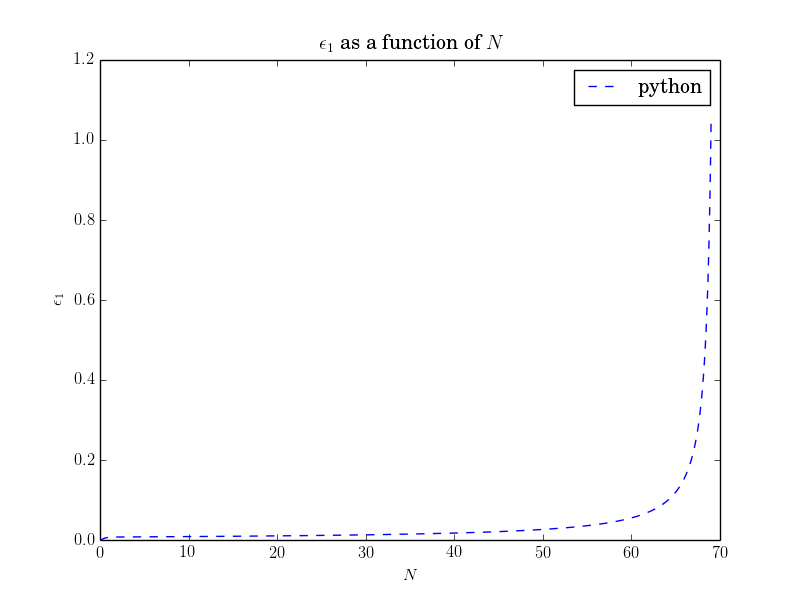
\includegraphics[scale=0.5]{eps1_vs_N.png}
\caption[Plot of $\epsilon 1(N)$ vs $N$ during power law inflation]{Plot of $\epsilon 1(N)$ vs $N$ during power law inflation}
\label{blah}
\end{center}
\end{figure}

\paragraph*{} Recall that the equation governing the tensor perturbations in the metric is

\begin{equation}
\ddot{h} + 3H\dot{h} - \frac{1}{a^2}\nabla ^2h = 0
\end{equation}

\noindent which, in fourier space, becomes

\begin{equation}
\ddot{h_k} + 3H\dot{h_k} + \frac{k^2}{a^2}h_k = 0
\end{equation}

\paragraph*{} Rewriting the above equation in terms of e-fold time, we arrive at

\begin{equation}
\frac{d^2h_k}{dN^2} + (3+\frac{1}{H}\frac{dH}{dN})\frac{dh_k}{dN} + \frac{k^2}{a^2H^2}h_k = 0
\end{equation}

\paragraph*{} The above equation was numerically integrated using a fourth order Runge-Kutta method, implemented in Python. It is to be noted that $h_k$ was evolved for various values of k, ranging from $10^{-6}$ to $10^{0}$. Corresponding initial and final limits on e-fold time N were placed by estimating the time when the modes are well inside the Hubble scale i.e $k/aH =  100$ and when the modes are well outside the Hubble scale i.e $k/aH =  10^{-5}$. The initial values for $h_k$ and $\frac{dh_k}{dN}$ were set to be

\begin{equation}
h_k  = \frac{1}{\sqrt{2k_0}a(N)}
\end{equation}

\begin{equation}
\frac{dh_k}{dN} = -\frac{1}{\sqrt{2k_0}a(N)} - \frac{i\sqrt{(k0/2)}}{a^2(N)H(N)}
\end{equation}

\paragraph*{} Having successfully obtained a numerical solution of $h_k$, we can evaluate the tensor power spectrum by using the formula

\begin{equation}
P_T(k) = 2 (\frac{k^3}{2\pi^2}) |h_k|^2
\end{equation}

\begin{figure}
\begin{center}
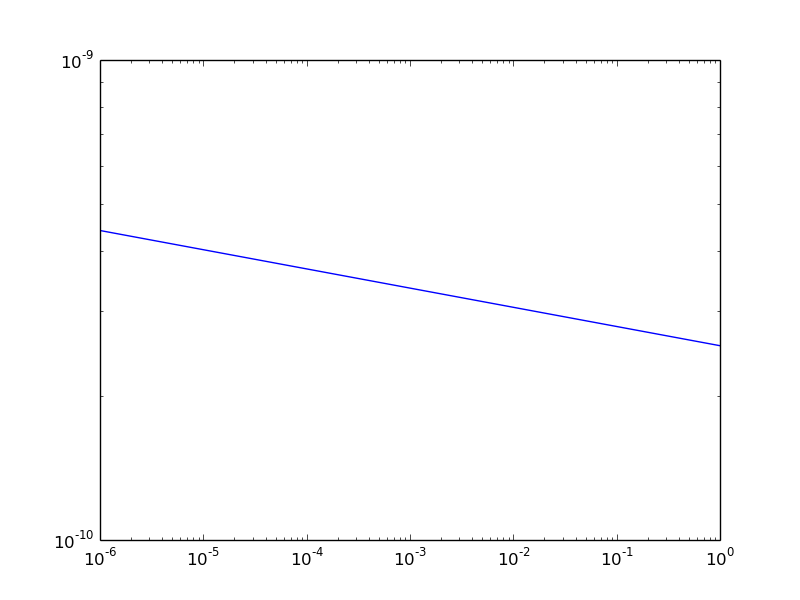
\includegraphics[scale=0.5]{power_spectrum_power_law.png}
\caption[Tensor power spectrum during power law inflation]{Tensor power spectrum during power law inflation}
\label{blah}
\end{center}
\end{figure}

\section{Small field inflation}

\paragraph*{} Similarly, if one considers the potential function that drives inflation to be of the form

\begin{equation}
V(\phi) = V_0(1-(\phi/\mu)^p)
\end{equation}

\noindent commonly referred to as small field inflation, the scalar field, the Hubble parameter and $\epsilon$ can all be numerically estimated to be

\begin{figure}
\begin{center}
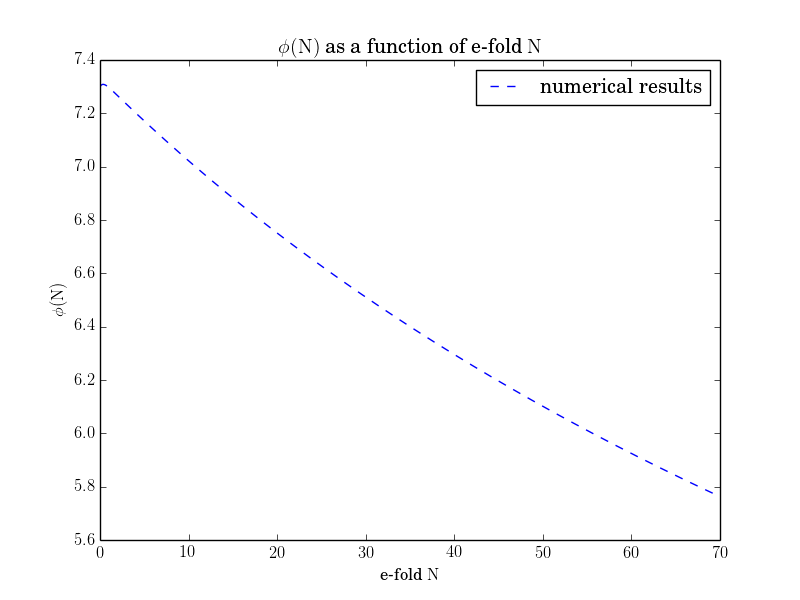
\includegraphics[scale=0.5]{phi_vs_N_small_field.png}
\caption[Plot of $\phi(N)$ vs $N$ during small field inflation]{Plot of $\phi(N)$ vs $N$ during small field inflation}
\label{blah}
\end{center}
\end{figure}

\begin{figure}
\begin{center}
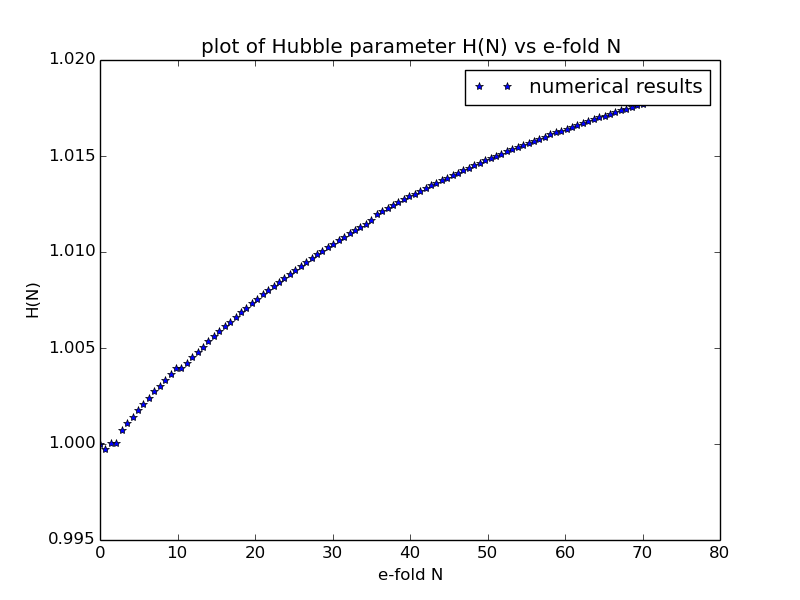
\includegraphics[scale=0.5]{H_vs_N_small_field.png}
\caption[Plot of $H(N)$ vs $N$ during small field inflation]{Plot of $H(N)$ vs $N$ during small field inflation}
\label{blah}
\end{center}
\end{figure}

\begin{figure}
\begin{center}
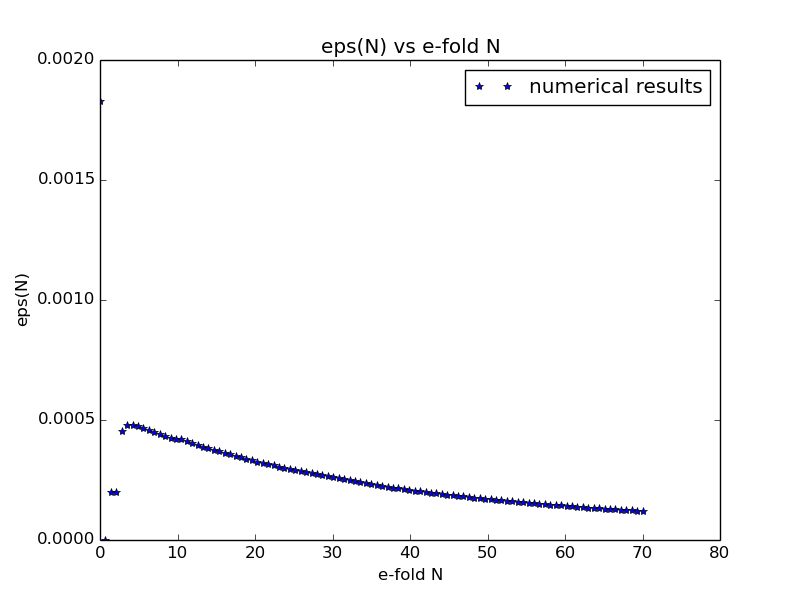
\includegraphics[scale=0.5]{eps1_vs_N_small_field.png}
\caption[Plot of $\epsilon 1(N)$ vs $N$ during small field inflation]{Plot of $\epsilon 1(N)$ vs $N$ during small field inflation}
\label{blah}
\end{center}
\end{figure}

%%%%%%%%%%%%%%%%%%%%%%%%%%%%%%%%%%%%%%%%%%%%%%%%%%%%%%%%%%%%%%%%%%%%%%%%%%%%%%%

\chapter{Summary}

%%%%%%%%%%%%%%%%%%%%%%%%%%%%%%%%%%%%%%%%%%%%%%%%%%%%%%%%%%%%%%%%%%%%%%%%%%%%%%%

\begin{thebibliography}{99}
%%%%%%%%%%%%%%%%%%%%%%%%%%%%%%%%%%%%%%%%%%%%%%%%%%%%%%%%%%%%%%%%%%%%%%%%%%%%%%%
\bibitem{Sriramkumar L - 2009}
L.~Sriramkumar, {\sl An introduction to inflation and cosmological perturbation theory}\/ (Current Science, 2009).
%%%%%%%%%%%%%%%%%%%%%%%%%%%%%%%%%%%%%%%%%%%%%%%%%%%%%%%%%%%%%%%%%%%%%%%%%%%%%%%
\end{thebibliography}
%%%%%%%%%%%%%%%%%%%%%%%%%%%%%%%%%%%%%%%%%%%%%%%%%%%%%%%%%%%%%%%%%%%%%%%%%%%%%%%

%\begin{appendices}
%\chapter{Python Code}
%\begin{verbatim}
%\end{verbatim}
%\end{appendices}
%%%%%%%%%%%%%%%%%%%%%%%%%%%%%%%%%%%%%%%%%%%%%%%%%%%%%%%%%%%%%%%%%%%%%%%%%%%%%%%
\end{document}